
We study the following descriptions of top quark pair production in the di-lepton channel:
%
\begin{description}
\item[~~~~~$\mathbf{NLO_{full}}$:]
  full NLO corrections to $pp\to W^+W^- b\bar{b}$ with leptonic $W$-decays,
\item[~~~~~$\mathbf{NLO_{NWA}^{NLOdec}}$:]
  NLO $t\bar{t}$ production $\otimes$ NLO decay,
\item[~~~~~$\mathbf{NLO_{NWA}^{LOdec}}$:]
  NLO $t\bar{t}$ production $\otimes$ LO decay,
\item[~~~~~$\mathbf{NLO_{PS}}$:]
  NLO $t\bar{t}$ production+shower $\otimes$ decay via parton showering.
\end{description}
We furthermore use the abbreviation $\mathbf{LO_{full}}$
for $W^+W^- b\bar{b}$ calculated at leading order, the abbreviation
$\mathbf{LO_{NWA}^{LOdec}}$ for LO $t\bar{t}$ production $\otimes$ LO
decay and the abbreviation $\mathbf{LO_{PS}}$ for LO $t\bar{t}$
production $\otimes$ decay via parton showering.
We investigate the effects of different levels in the description
of the top quark decay,
isolating the latter from the effects of the non-resonant and
non-factorisable contributions contained in the $\nlofull$ calculation.
This is done by emulating a concrete experimental analysis used for top
quark mass determinations.
As we match to a parton shower, i.e.~use $\nlops$ only in the
factorised case, we do not need to address the problem of
``resonance-aware matching''~\cite{Jezo:2016ujg,Frederix:2016rdc}.
This allows us to get a clear idea of the effects of the various
approximations used here, which in turn can serve as a basis for
future studies entirely relying on showered results.

The calculations $\nlofull$ and $\lodec$ have been already described
in detail in Ref.~\cite{Heinrich:2013qaa}.\footnote{%
  In Ref.~\cite{Heinrich:2013qaa}, $\nlofull$ was called
  $W^+W^- b\bar{b}$ and $\lodec$ was called $t\bar{t}$.}
Here we briefly summarise only the main features. We use
\tsc{GoSam}~\cite{Cullen:2011ac,Cullen:2014yla} plus
\tsc{Sherpa}~\cite{Gleisberg:2008ta}, version 2.2.3, where the virtual
corrections generated by \tsc{GoSam} are linked to \tsc{Sherpa} via
the Binoth-Les-Houches-interface~\cite{Binoth:2010xt,Alioli:2013nda}.
This applies not only to the calculations $\nlofull$ and $\lodec$ but
also to the $\nlops$ computation. We note that our full NLO
calculation of the process $pp\rightarrow W^+W^-b\bar b\rightarrow
(e^+ \nu_e)\,(\mu^- \bar{\nu}_{\mu})\,b\bar b$ provides a complete
description of the final state including singly-resonant and
non-resonant top quark contributions. Example diagrams are shown in
Fig.~\ref{fig:wwbb_diagrams}. The computation relies on the
5-flavour scheme, i.e.~the $b$-quark is treated as massless.
To take the top quark decay width into account in a gauge invariant
way, the complex mass scheme~\cite{Denner:2006ic} is used. In our
setup, this amounts to a replacement of the top quark mass by a
complex number $\mu_t$ evaluated according to
\begin{equation}
\mu_t^2\;=\;m_t^2-i\,m_t\,\Gamma_t~.
\label{eq:cms}
\end{equation}
The weak mixing angle remains real-valued in our calculation, as we
neglect non-resonant $W$ and $Z$-boson contributions.

\begin{figure}[tbp!]
  \centering
  \begin{subfigure}[b]{0.4\textwidth}
    \centering
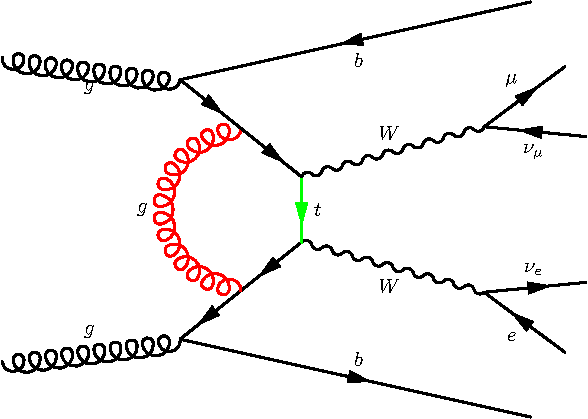
\includegraphics[width=1\textwidth]{{plots/virt1}.pdf}
  \end{subfigure}
  \hskip10mm
  \begin{subfigure}[b]{0.4\textwidth}
    \centering
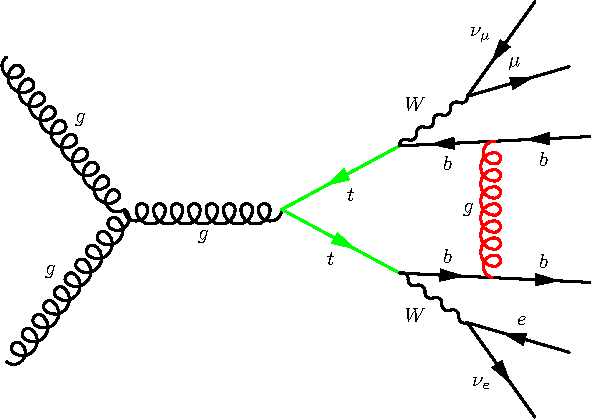
\includegraphics[width=1\textwidth]{{plots/virt2}.pdf}
  \end{subfigure}
  \caption{\label{fig:wwbb_diagrams}
    Examples of one-loop Feynman diagrams contributing to the
    $\nlofull$ calculation, i.e.~the full
    $W^+W^-b\bar{b}$ calculation at NLO: two diagrams are shown
    depicting a non-resonant (left) and a   
    non-factorisable virtual contribution (right).}
\end{figure}
%
The results for the $\nlodec$ calculation are obtained
as described in Ref.~\cite{Melnikov:2009dn}.\footnote{%
  The corresponding Monte Carlo generator is publicly available at
  {\tt https://github.com/ TOPAZdevelop/TOPAZ}.}
This framework relies on the factorisation of the matrix elements according to
\begin{eqnarray}\label{eqn:NWA1}
   \mathcal{M}^\mathrm{NWA}_{ij\to t\bar{t}\to b \bar{b} 2l 2\nu}
   \;=\;
   \mathcal{P}_{ij \to t\bar{t}} \otimes \mathcal{D}_{t\to b l^+ \nu}
   \otimes \mathcal{D}_{\bar{t}\to \bar{b} l^- \bar{\nu}}~,
\end{eqnarray}
where $\mathcal{P}_{ij \to t\bar{t}}$ describes the $t\bar{t}$ production process and $\mathcal{D}_{t\to b l \nu}$ the top quark decay dynamics.
Spin correlations are included as indicated by the symbol $\otimes$.
Squaring Eq.~(\ref{eqn:NWA1}) and integrating over the phase space yields the
double-resonant partonic cross section
\begin{eqnarray}\label{eqn:sigmaNWA}
\hat{\sigma}_{ij\to b \bar{b} 2l 2\nu}\;=\;\int \!\! \mathrm{d}\mathrm{PS} \; |\mathcal{M}^\mathrm{NWA}_{ij\to t\bar{t}\to b \bar{b} 2l 2\nu}|^2
+ \mathcal{O}\left(\Gamma_t\big/ m_t\right)
\end{eqnarray}
where off-shell effects are parametrically suppressed by $\Gamma_t \big/ m_t \approx 0.7 \%$.
Expanding Eq.~(\ref{eqn:NWA1}) up to NLO yields
\begin{eqnarray}\label{eqn:NWA2}
   \mathcal{M}^\mathrm{NWA,\; NLO}_{ij\to t\bar{t}\to b \bar{b} 2l 2\nu}
   =&&
   \mathcal{P}_{ij \to t\bar{t}}^\mathrm{LO} \otimes \mathcal{D}^\mathrm{LO}_{t\to b l^+ \nu} \otimes \mathcal{D}^\mathrm{LO}_{\bar{t}\to \bar{b} l^- \bar{\nu}}
  +\mathcal{P}_{ij \to t\bar{t}}^{\delta \mathrm{NLO}} \otimes \mathcal{D}^\mathrm{LO}_{t\to b l^+ \nu} \otimes \mathcal{D}^\mathrm{LO}_{\bar{t}\to \bar{b} l^- \bar{\nu}}
    \nonumber  \\
   +&&
   \mathcal{P}_{ij \to t\bar{t}}^\mathrm{LO} \otimes \left( \mathcal{D}^{\delta \mathrm{NLO}}_{t\to b l^+ \nu} \otimes \mathcal{D}^\mathrm{LO}_{\bar{t}\to \bar{b} l^- \bar{\nu}}
   +\mathcal{D}^\mathrm{LO}_{t\to b l^+ \nu} \otimes \mathcal{D}^{\delta \mathrm{NLO}}_{\bar{t}\to \bar{b} l^- \bar{\nu}} \right)~.
\end{eqnarray}
The NLO corrections to the production process $\mathcal{P}_{ij \to t\bar{t}}^{\delta \mathrm{NLO}}$ involve the virtual and real emission matrix elements
$\mathcal{M}_{gg/q\bar{q} \to t\bar{t}}^{\mathrm{virt}}$, $\mathcal{M}_{gg/q\bar{q} \to t\bar{t}+g}^{\mathrm{real}}$ and
$\mathcal{M}_{qg/\bar{q}g \to t\bar{t}+q/\bar{q}}^{\mathrm{real}}$.
The corresponding NLO decay parts are given by
\begin{eqnarray}\label{eqn:NWAdecay}
\mathcal{D}^\mathrm{virt (real)}_{t\to b l \nu}\;=\;\frac{\mathcal{M}^\mathrm{virt (real)}_{t\to b W (+g)}}{\sqrt{2 m_t \Gamma_t^\mathrm{NLO}}} \otimes
\frac{\mathcal{M}_{W \to l \nu}}{\sqrt{2 M_W  \Gamma_W^\mathrm{NLO}}}~.
\end{eqnarray}
We note that, in contrast to Ref.~\cite{Melnikov:2009dn}, the top quark width $\Gamma_t^\mathrm{NLO}$ in the denominator is not expanded
as $(\Gamma_t^\mathrm{NLO})^{-1/2}=(\Gamma_t^\mathrm{LO})^{-1/2}
\left( 1 - 1/2 \, \alpha_s \, \Gamma_t^{\delta
    \mathrm{NLO}}/\Gamma_t^\mathrm{LO} \right) $, analogously for $(\Gamma_W^\mathrm{NLO})^{-1/2}$.

For our studies relying on $\lodec$ results, we remove all
contributions in the second line of Eq.~(\ref{eqn:NWA2}) and use
$\Gamma_{t,W}^\mathrm{LO}$ instead of $\Gamma_{t,W}^\mathrm{NLO}$. This
treatment guarantees that
$\int \! \mathrm{d}\mathrm{PS} \; |\mathcal{D}_{t\to b l \nu}|^2 =
\mathrm{BR}(t\to bl\nu)$ at LO and NLO, with $\mathrm{BR}(t\to bl\nu)$
denoting the branching ratio for the top quark decay.


Finally, the $\nlops$ computations are based on the
NLO plus parton-shower matching scheme as implemented in
\tsc{Sherpa}~\cite{Hoeche:2011fd}. The original scheme was extended in
Ref.~\cite{Hoeche:2013mua} to incorporate heavy-quark mass effects.
Utilising this scheme, we obtain an NLO+PS accurate description of
$t\bar t$+jets, or, in other words, the NLO description of the
$t\bar t$ production shower. The top quark decays are attached
afterwards such that LO spin correlations are preserved, and each decay
configuration is supplemented by its respective decay shower following
the same procedure as described in Ref.~\cite{Hoche:2014kca}.
For our investigations, we used \tsc{Sherpa}~version~\tsc{2.2.3}.
In the course of this work, it was found that this version treats
radiation emerging from top quark decays in resonant top quark
processes in the same manner as radiation arising from continuum
production processes. This resulted in an omission of the
initial-state spectator mass term that suppresses the ordinary eikonal
radiation of continuum initial-final dipoles.
The problem has been identified and solved by
the implementation of a dedicated dipole-shower algorithm for the
decays, similar to Ref.~\cite{Hamilton:2006ms}. The patch implementing
these changes has been provided by the \tsc{Sherpa} authors and was
used for our results presented below. It will be made available on the
corresponding software download pages, and included in the
\tsc{Sherpa} program from version~\tsc{2.2.5} onwards.

